\subsection{商群的子群与商群}

设 G 是一个拓扑群，H 是 G 的一个正规子群，\(\varphi: G \to G/H\) 是典范映射。我们知道，若 \(A'\) 是 G/H 的一个子群，则 \(\varphi^{-1}(A')\) 是 G 的一个包含 H 的子群。反之，若 A 是 G 的一个子群，则 \(\varphi(A)\) 是 G/H 的一个子群；此外，存在商群 \(A/(A \cap H)\) 到 G/H 的子群 \(\varphi(A)\) 上的一个典范双射，以及 \(\varphi(A)\) 到商群 AH/H 上的一个典范双射，且这两个双射对群结构而言都是同构。

命题 20 设 A 是拓扑群 G 的一个子群，H 是 G 的一个正规子群，\(\varphi\) 表示 G 到 G/H 上的典范映射。则 \(\varphi(A)\) 到 AH/H 上的典范双射是拓扑群的一个同构。

这由前面的注记以及第 4 目命题 10 得出。

\pandocbounded{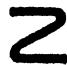
\includegraphics[keepaspectratio]{images/part002_0097f9c2.jpg}}

\(\mathbf{A}/(\mathbf{A} \cap \mathbf{H})\) 到 \(\varphi(\mathbf{A})\) 上的典范双射是连续同态，因为它是由 \(\varphi\) 在 \(\mathbf{A}\) 上的限制过渡到商而产生的；但一般地说，拓扑群 \(\mathbf{A}/(\mathbf{A} \cap \mathbf{H})\) 与 \(\mathbf{AH}/\mathbf{H}\) 不同构（参看 § 4 第 1 目命题 1 推论 3）。

* 例如，取 G 为实数的加法群 R，取 H 为整数群 Z，取 A 为一个无理数 θ 的整数倍组成的群 θZ。则 A∩H = \{0\}，因而 A/(A∩H) 是一个离散群，同构于 Z；另一方面，A + H 在 R 中稠密（我们将在第五章 § 1 第 1 目命题 1 中看到），于是 (A + H)/H——它与 A + H 局部同构（第 6 目命题 19）——不是离散群，从而不同构于 A/(A∩H)。*

尽管如此，我们有下面的命题：

命题 21 设 G 是一个拓扑群，\(G_{0}\) 是 G 的一个稠密子群，\(H_{0}\) 是 \(G_{0}\) 的一个正规子群，H 是 \(H_{0}\) 在 G 中的闭包，\(\varphi\) 是典范映射 \(G \rightarrow G/H\)。则典范双射 \(G_{0}/H_{0} \rightarrow \varphi(G_{0})\) 是拓扑群 \(G_{0}/H_{0}\) 到 G/H 的一个稠密子群上的一个同构。

由于 \(\mathbf{H}_0 = \mathbf{H} \cap \mathbf{G}_0\)，只需证明：若 \(\mathbf{U}_0\) 是 \(\mathbf{G}_0\) 的任一开子集，它关于关系 \(x^{-1}y \in \mathbf{H}_0\) 是饱和的，则 \(\mathbf{U}_0\) 是 \(\mathbf{G}_0\) 与 \(\mathbf{G}\) 的一个关于关系 \(x^{-1}y \in \mathbf{H}\) 饱和的开子集的交（第一章 § 3 第 6 目命题 10）。设 \(\mathbf{U}\) 是 \(\mathbf{G}\) 的一个使 \(\mathbf{U}_0 = \mathbf{U} \cap \mathbf{G}_0\) 的开子集。由于 \(\mathbf{U}_0 = \mathbf{U}_0\mathbf{H}_0\)，容易看出 \(\mathbf{U}_0 = \mathrm{UH}_0 \cap \mathbf{G}_0\)；但 \(\mathrm{UH}_0\) 在 \(\mathbf{G}\) 中是开的，故可设 \(\mathbf{U} = \mathrm{UH}_0\)。集合 \(\mathrm{UH}\) 在 \(\mathbf{G}\) 中是开的且关于关系 \(x^{-1}y \in \mathbf{H}\) 是饱和的；因此只要证明 \(\mathrm{UH} \cap \mathbf{G}_0 = \mathbf{U}_0\)，命题就证明了。现在，若 \(u \in \mathbf{U}\) 与 \(h \in \mathbf{H}\) 使 \(uh \in \mathbf{G}_0\)，则存在一个对称邻域 \(\mathbf{V}\)（\(e\) 在 \(\mathbf{G}\) 中的），使得 \(uv \subset U\)；由于 \(Vh\) 是 \(h\) 在 \(\mathbf{G}\) 中的一个邻域，存在 \(z \in V\) 使 \(zh \in \mathbf{H}_0\)。于是有 \(uz^{-1} \in U\)，且 \(uh = (uz^{-1})(zh)\)；因此 \(\mathrm{UH} \cap \mathbf{G}_0 \subset \mathrm{UH}_0\)。但 \(\mathrm{UH}_0 = U\)，于是 \(\mathrm{UH} \cap \mathbf{G}_0 \subset U \cap \mathbf{G}_0 = U_0\)。证毕。

设 G 是连续作用在拓扑空间 X 上的一个拓扑群，K 是 G 的一个正规子群，它含于 X 的每一点的稳定子群中。对每个 \(x \in X\)，关系 \(s \equiv t \pmod{K}\) 因而蕴含 s.x = t.x，并且过渡到商，我们定义一个 G/K 到 X 中的映射 \(\dot{s} \to \dot{s}.x\)。立即可验证，关于外法则 \((\dot{s}, x) \to \dot{s}.x\)，X 以 G/K 为算子群。此外，G/K 关于这个法则连续作用在 X 上；因为 X 上的相等关系与 G 上的关系 \(s \equiv t \pmod{K}\) 都是开的等价关系，于是结论由映射

\[
(s, x) \rightarrow \dot {s}. x = s. x
\]

（\(\mathbf{G} \times \mathbf{X}\) 到 \(\mathbf{X}\) 中的）的连续性得出（第一章 § 5 第 3 目命题 8 的推论，以及 § 3 第 4 目命题 6）。

现设 G 是连续作用在拓扑空间 X 上的一个拓扑群，H 是 G 的任一正规子群；则 H 连续作用在 X 上。设 S 是 H 在 X 上定义的等价关系；则 S 是开的（第 4 目引理 2）。关系 S 与群 G 相容（第 4 目）；因为若 \(y \equiv x \pmod{S}\)，则存在 \(t \in H\) 使 y = t.x；于是对所有 \(s \in G\) 有 \(s.y = (sts^{-1}) \cdot s.x\)，且由于 H 在 G 中正规，有 \(sts^{-1} \in H\)；从而 \(s.y \equiv s.x \pmod{S}\)。若 \(\psi\) 是 X 到 X/S 上的典范映射，则群 G 关于外法则

\[
(s, \psi (x)) \rightarrow \psi (s. x)
\]

（第 4 目命题 11）。此外，群 H 含于 X/S 的每一点的稳定子群中；如我们上面所见，G/H 关于外法则 \((s, \psi(x)) \to \psi(s.x)\) 连续作用在 X/S = X/H 上。若 R 表示 G 在 X 上定义的等价关系，则关系 S 蕴含 R，且 X/S 上的等价关系 R/S 是由群 G/H 定义的。因此（第一章 § 3 第 4 目命题 7）：

命题 22 设 G 是连续作用在拓扑空间 X 上的一个拓扑群，H 是 G 的一个正规子群。则 X/G 到 (X/H)/(G/H) 上的典范双射是一个同胚。

推论 设 G 是一个拓扑群，H 是 G 的一个正规子群，K 是 G 的一个包含 H 的正规子群。则 G/K 到 (G/H)/(K/H) 上的典范双射是拓扑群的一个同构。

我们已知道这个双射是群的一个同构，而命题 22（应用于在 G 的右边作用的群 K）表明它是一个同胚。

